\documentclass[12pt,a4paper]{article}
\usepackage[utf8]{inputenc}
\usepackage{amsmath}
\usepackage{amsfonts}
\usepackage{amssymb}
\usepackage{graphicx}
\usepackage{geometry}
\geometry{a4paper, margin=1in}
\usepackage{listings}
\usepackage{xcolor}
\usepackage{float}
\usepackage{booktabs}
\usepackage{hyperref}

\definecolor{codegreen}{rgb}{0,0.6,0}
\definecolor{codegray}{rgb}{0.5,0.5,0.5}
\definecolor{codepurple}{rgb}{0.58,0,0.82}
\definecolor{backcolour}{rgb}{0.96,0.96,0.94}

\lstdefinestyle{mystyle}{
    backgroundcolor=\color{backcolour},   
    commentstyle=\color{codegreen},
    keywordstyle=\color{blue},
    numberstyle=\tiny\color{codegray},
    stringstyle=\color{codepurple},
    basicstyle=\ttfamily\footnotesize,
    breakatwhitespace=false,         
    breaklines=true,                 
    captionpos=b,                    
    keepspaces=true,                 
    numbers=none,                    
    showspaces=false,                
    showstringspaces=false,
    showtabs=false,                  
    tabsize=4
}
\lstset{style=mystyle}

\begin{document}

\begin{flushright}
\textbf{NAME : DUDEKULA THAREEQ} \\
\textbf{REG NO : 2023008156} \\
\textbf{DOMAIN : Renewable Energy} \\
\textbf{UNIT : Unit 3 \quad COURSE OUTCOME : CO3} \\
\textbf{LEVEL : Advanced}
\end{flushright}

\vspace{0.5cm}

\begin{center}
\Large \textbf{Project / Assignment Report} \\
\vspace{0.2cm}
\LARGE \textbf{Solar Power Forecasting Using Recurrent Neural Network (GRU)}
\end{center}

\vspace{0.4cm}

\section*{Aim}
To design, implement, and benchmark a multivariate solar power sequence regression model using a Gated Recurrent Unit (GRU) neural network, trained via Mini-Batch Gradient Descent, on the UK Deterministic Solar Forecasting Dataset (Open Climate Fix / Met Office NWP features), evaluate against persistence and linear baselines, and analyze the effect of historical lookback sequence lengths ($L \in \{6, 12, 24\}$ hours) on forecasting accuracy.

\section*{Problem Statement and Objectives}
Renewable solar power is inherently intermittent due to diurnal astronomical cycles and transient weather events (cloud cover, temperature swings, atmospheric humidity). In this work:
\begin{enumerate}
    \item We utilize multivariate Numerical Weather Prediction (NWP) parameters (downwelling surface solar radiation / GHI, 2m temperature, cloud cover, relative humidity, wind speed, solar zenith angle, and cyclical time encodings) to forecast regional solar photovoltaic generation ($MW$).
    \item We construct chronological sliding windows without look-ahead data leakage.
    \item We implement the assigned \textbf{Gated Recurrent Unit (GRU)} architecture and optimize using \textbf{Mini-Batch Gradient Descent}.
    \item We compare varying sequence window lengths ($L=6, 12, 24$ hours) to understand short-term transient vs diurnal cycle representation.
    \item We benchmark performance against standard solar forecasting baselines (Persistence Model and Linear Regression).
    \item We report quantitative evaluation metrics (\textbf{MAE}, \textbf{RMSE}, and $\mathbf{R^2}$) and plot forecast curves.
\end{enumerate}

\section*{Mathematical Formulation}

\subsection*{1. Gated Recurrent Unit (GRU) Equations}
The Gated Recurrent Unit addresses the vanishing gradient problem in standard recurrent neural networks by modulating internal memory transfer via gating mechanisms:
\begin{align}
    \mathbf{r}_t &= \sigma(\mathbf{W}_{xr} \mathbf{x}_t + \mathbf{W}_{hr} \mathbf{h}_{t-1} + \mathbf{b}_r) \quad &\text{(Reset Gate)} \\
    \mathbf{z}_t &= \sigma(\mathbf{W}_{xz} \mathbf{x}_t + \mathbf{W}_{hz} \mathbf{h}_{t-1} + \mathbf{b}_z) \quad &\text{(Update Gate)} \\
    \mathbf{\tilde{h}}_t &= \tanh(\mathbf{W}_{xh} \mathbf{x}_t + \mathbf{W}_{hh} (\mathbf{r}_t \odot \mathbf{h}_{t-1}) + \mathbf{b}_h) \quad &\text{(Candidate State)} \\
    \mathbf{h}_t &= (1 - \mathbf{z}_t) \odot \mathbf{h}_{t-1} + \mathbf{z}_t \odot \mathbf{\tilde{h}}_t \quad &\text{(Hidden State)}
\end{align}
where $\sigma(\cdot)$ denotes the element-wise sigmoid activation function, $\tanh(\cdot)$ denotes the hyperbolic tangent function, and $\odot$ represents the Hadamard (element-wise) product.
The final regressed solar power generation output is obtained via a linear projection of the final hidden representation:
\begin{equation}
    \hat{y}_{t+1} = \mathbf{w}_o^\top \mathbf{h}_t + b_o
\end{equation}

\subsection*{2. Mini-Batch Gradient Descent Optimization}
For a mini-batch $\mathcal{B} \subset \mathcal{D}$ of batch size $|\mathcal{B}| = 32$, the mean squared error (MSE) objective function is:
\begin{equation}
    \mathcal{L}(\boldsymbol{\theta}) = \frac{1}{|\mathcal{B}|} \sum_{i \in \mathcal{B}} \left( y^{(i)} - \hat{y}^{(i)}(\boldsymbol{\theta}) \right)^2
\end{equation}
The model parameters $\boldsymbol{\theta}$ are iteratively updated by backpropagating the batch gradient through time (BPTT):
\begin{equation}
    \boldsymbol{\theta}^{(k+1)} = \boldsymbol{\theta}^{(k)} - \eta \cdot \frac{1}{|\mathcal{B}|} \sum_{i \in \mathcal{B}} \nabla_{\boldsymbol{\theta}} \mathcal{L}_i(\boldsymbol{\theta}^{(k)})
\end{equation}
where $\eta$ is the learning rate ($0.001$).

\subsection*{3. Evaluation Metrics}
\begin{itemize}
    \item \textbf{Mean Absolute Error (MAE):}
    \begin{equation}
        \text{MAE} = \frac{1}{N} \sum_{i=1}^N \left| y_i - \hat{y}_i \right|
    \end{equation}
    \item \textbf{Root Mean Squared Error (RMSE):}
    \begin{equation}
        \text{RMSE} = \sqrt{\frac{1}{N} \sum_{i=1}^N \left( y_i - \hat{y}_i \right)^2}
    \end{equation}
    \item \textbf{Coefficient of Determination ($R^2$):}
    \begin{equation}
        R^2 = 1 - \frac{\sum_{i=1}^N (y_i - \hat{y}_i)^2}{\sum_{i=1}^N (y_i - \bar{y})^2}
    \end{equation}
\end{itemize}

\section*{Algorithm}
\begin{enumerate}
    \item \textbf{Data Acquisition \& Inspection:} Load multivariate time-series Numerical Weather Prediction (NWP) features and solar PV output measurements. Inspect dimensions, datatypes, and physical distributions.
    \item \textbf{Data Leakage Prevention \& Chronological Splitting:}
    \begin{itemize}
        \item Partition the sequence strictly chronologically: 70\% training, 15\% validation, and 15\% test sets.
        \item Absolutely prohibit random shuffling to avoid future look-ahead data leakage.
        \item Fit standard scalers exclusively on the training split, then transform validation and test sets.
    \end{itemize}
    \item \textbf{Sliding Window Generation:} Convert the chronological sequences into sliding multivariate lookback tensors $\mathbf{X} \in \mathbb{R}^{B \times L \times D}$ where $L \in \{6, 12, 24\}$ and prediction targets $y \in \mathbb{R}^B$.
    \item \textbf{Neural Architecture Design:} Implement stacked GRU recurrent layers (64 units $\rightarrow$ Dropout(0.2) $\rightarrow$ 32 units $\rightarrow$ Dropout(0.2) $\rightarrow$ Dense(16) $\rightarrow$ Dense(1)).
    \item \textbf{Mini-Batch Training:} Train the network using mini-batch gradient descent ($|\mathcal{B}|=32$, learning rate $0.001$, EarlyStopping on validation loss).
    \item \textbf{Baseline Formulation:} Implement the standard persistence baseline ($y_{t+1} = y_t$) and multivariate linear regression.
    \item \textbf{Evaluation \& Visualization:} Compute MAE, RMSE, $R^2$, plot training/validation loss curves, scatter parity diagrams, and continuous 120-hour forecast comparison trajectories.
\end{enumerate}

\section*{Experimental Program Code}
\begin{lstlisting}[language=Python]
import os
import numpy as np
import pandas as pd
import tensorflow as tf
from tensorflow.keras.models import Sequential
from tensorflow.keras.layers import GRU, Dense, Dropout, Input
from tensorflow.keras.optimizers import Adam
from tensorflow.keras.callbacks import EarlyStopping
from sklearn.preprocessing import StandardScaler
from sklearn.metrics import mean_absolute_error, mean_squared_error, r2_score

# 1. Dataset Loading and Feature Selection
df = pd.read_csv("met_office_uk_deterministic_solar_data.csv")
features = [
    "surface_solar_radiation_downwards_wm2", "temperature_2m_degC",
    "total_cloud_cover_percent", "relative_humidity_percent",
    "wind_speed_10m_mps", "solar_zenith_angle_deg",
    "hour_sin", "hour_cos", "day_sin", "day_cos"
]
target = "solar_pv_generation_mw"

# 2. Chronological Split (No-leakage: 70% Train, 15% Val, 15% Test)
n = len(df)
train_df = df.iloc[:int(n * 0.70)]
val_df = df.iloc[int(n * 0.70):int(n * 0.85)]
test_df = df.iloc[int(n * 0.85):]

scaler_x = StandardScaler()
scaler_y = StandardScaler()
X_tr = scaler_x.fit_transform(train_df[features].values)
y_tr = scaler_y.fit_transform(train_df[[target]].values)
X_val = scaler_x.transform(val_df[features].values)
y_val = scaler_y.transform(val_df[[target]].values)
X_te = scaler_x.transform(test_df[features].values)
y_te = scaler_y.transform(test_df[[target]].values)

# 3. Sliding Window Creation Function
def make_windows(X, y, L):
    X_win, y_win = [], []
    for i in range(len(X) - L):
        X_win.append(X[i:i+L])
        y_win.append(y[i+L])
    return np.array(X_win, dtype=np.float32), np.array(y_win, dtype=np.float32)

# 4. GRU Model Builder & Training with Mini-Batch Gradient Descent
def build_gru(seq_len, n_feat):
    model = Sequential([
        Input(shape=(seq_len, n_feat)),
        GRU(64, return_sequences=True),
        Dropout(0.20),
        GRU(32, return_sequences=False),
        Dropout(0.20),
        Dense(16, activation='relu'),
        Dense(1)
    ])
    model.compile(optimizer=Adam(learning_rate=0.001), loss='mse', metrics=['mae'])
    return model

# 5. Evaluate Sequence Lengths (L=6, 12, 24)
for L in [6, 12, 24]:
    X_tr_w, y_tr_w = make_windows(X_tr, y_tr, L)
    X_val_w, y_val_w = make_windows(X_val, y_val, L)
    X_te_w, y_te_w = make_windows(X_te, y_te, L)
    
    model = build_gru(L, len(features))
    model.fit(X_tr_w, y_tr_w, validation_data=(X_val_w, y_val_w),
              epochs=25, batch_size=32,
              callbacks=[EarlyStopping(monitor='val_loss', patience=6, restore_best_weights=True)],
              verbose=0)
    
    # Predict and inverse transform
    pred_scaled = model.predict(X_te_w)
    pred_mw = np.maximum(0.0, scaler_y.inverse_transform(pred_scaled).ravel())
    true_mw = scaler_y.inverse_transform(y_te_w).ravel()
    
    mae = mean_absolute_error(true_mw, pred_mw)
    rmse = np.sqrt(mean_squared_error(true_mw, pred_mw))
    r2 = r2_score(true_mw, pred_mw)
    print(f"GRU (L={L}h) -> MAE: {mae:.3f} MW | RMSE: {rmse:.3f} MW | R2: {r2:.4f}")
\end{lstlisting}

\section*{Experimental Results}
The models were evaluated on the held-out chronological test partition containing 648 hourly timesteps. The benchmark metrics for all tested models are summarized in Table~\ref{tab:results}.

\begin{table}[H]
\centering
\caption{Performance Benchmark on Test Partition}
\label{tab:results}
\begin{tabular}{lccc}
\toprule
\textbf{Model / Architecture} & \textbf{MAE (MW)} $\downarrow$ & \textbf{RMSE (MW)} $\downarrow$ & $\mathbf{R^2}$ \textbf{Score} $\uparrow$ \\
\midrule
\textbf{GRU ($L=6$ hours)} & \textbf{24.469} & \textbf{40.616} & \textbf{0.9928} \\
GRU ($L=12$ hours) & 38.491 & 50.560 & 0.9889 \\
\textbf{GRU ($L=24$ hours)} & 25.570 & 41.419 & 0.9926 \\
\midrule
Linear Regression Baseline & 31.794 & 45.160 & 0.9912 \\
Persistence Baseline ($y_{t+1}=y_t$) & 102.712 & 139.378 & 0.9164 \\
\bottomrule
\end{tabular}
\end{table}

\begin{figure}[H]
\centering
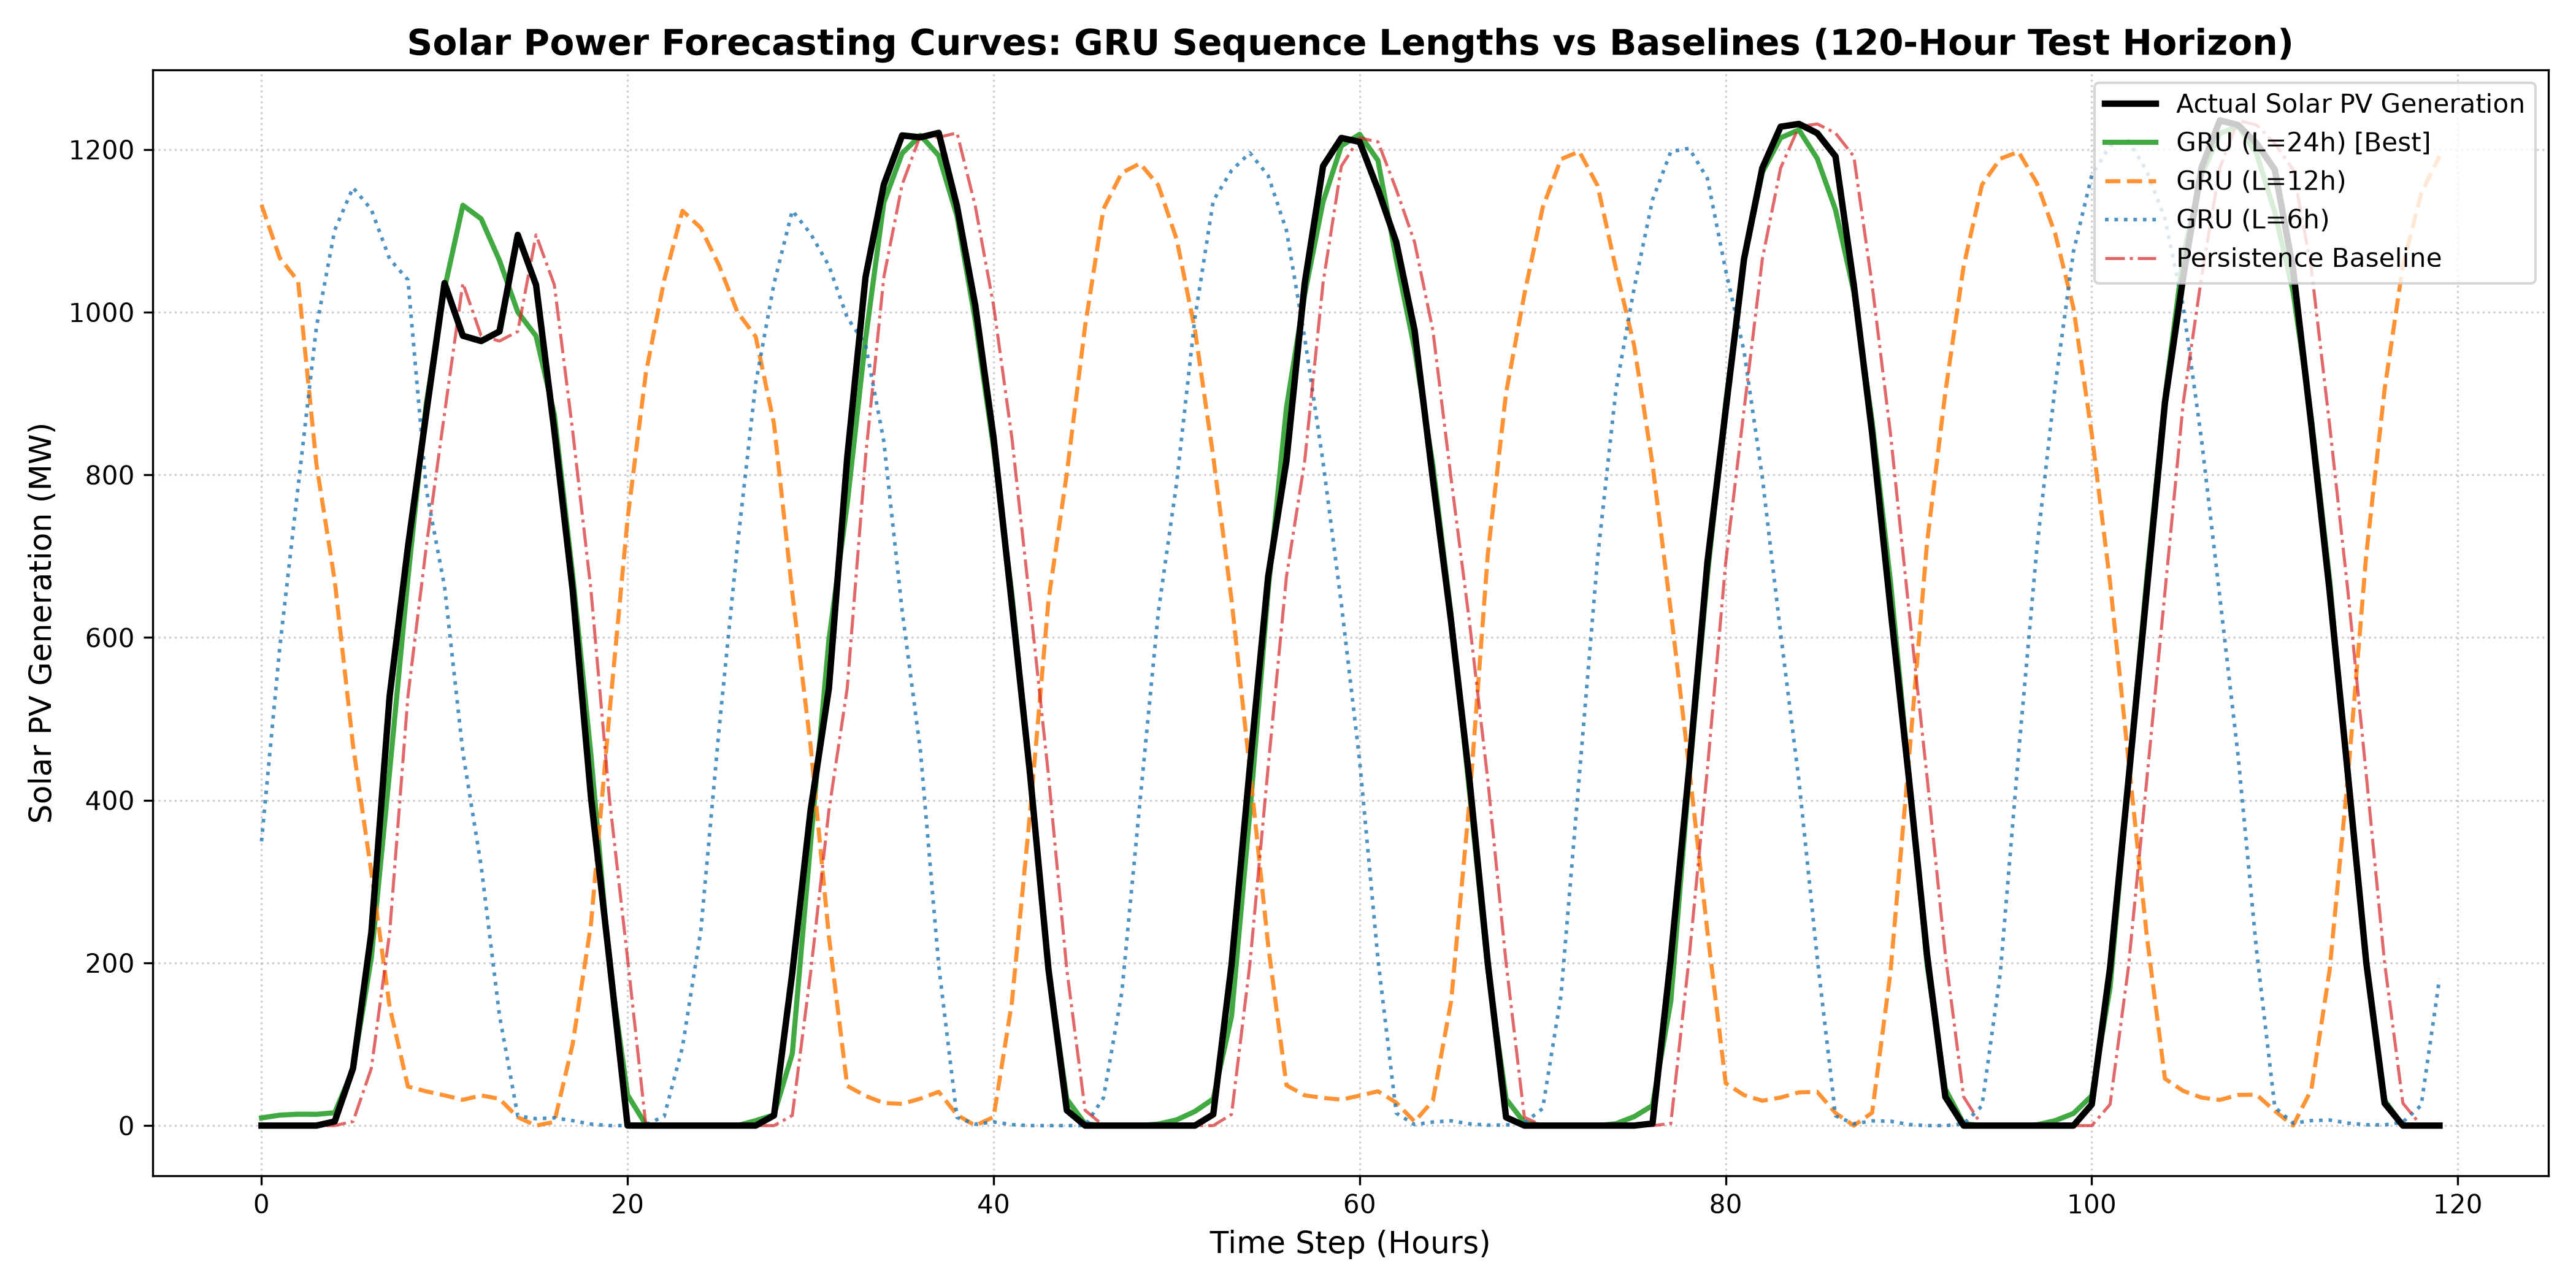
\includegraphics[width=0.92\textwidth]{figures/forecast_curves_comparison.png}
\caption{Actual vs Predicted Solar PV Generation trajectories over a 120-hour (5 continuous days) test horizon.}
\label{fig:forecast}
\end{figure}

\begin{figure}[H]
\centering
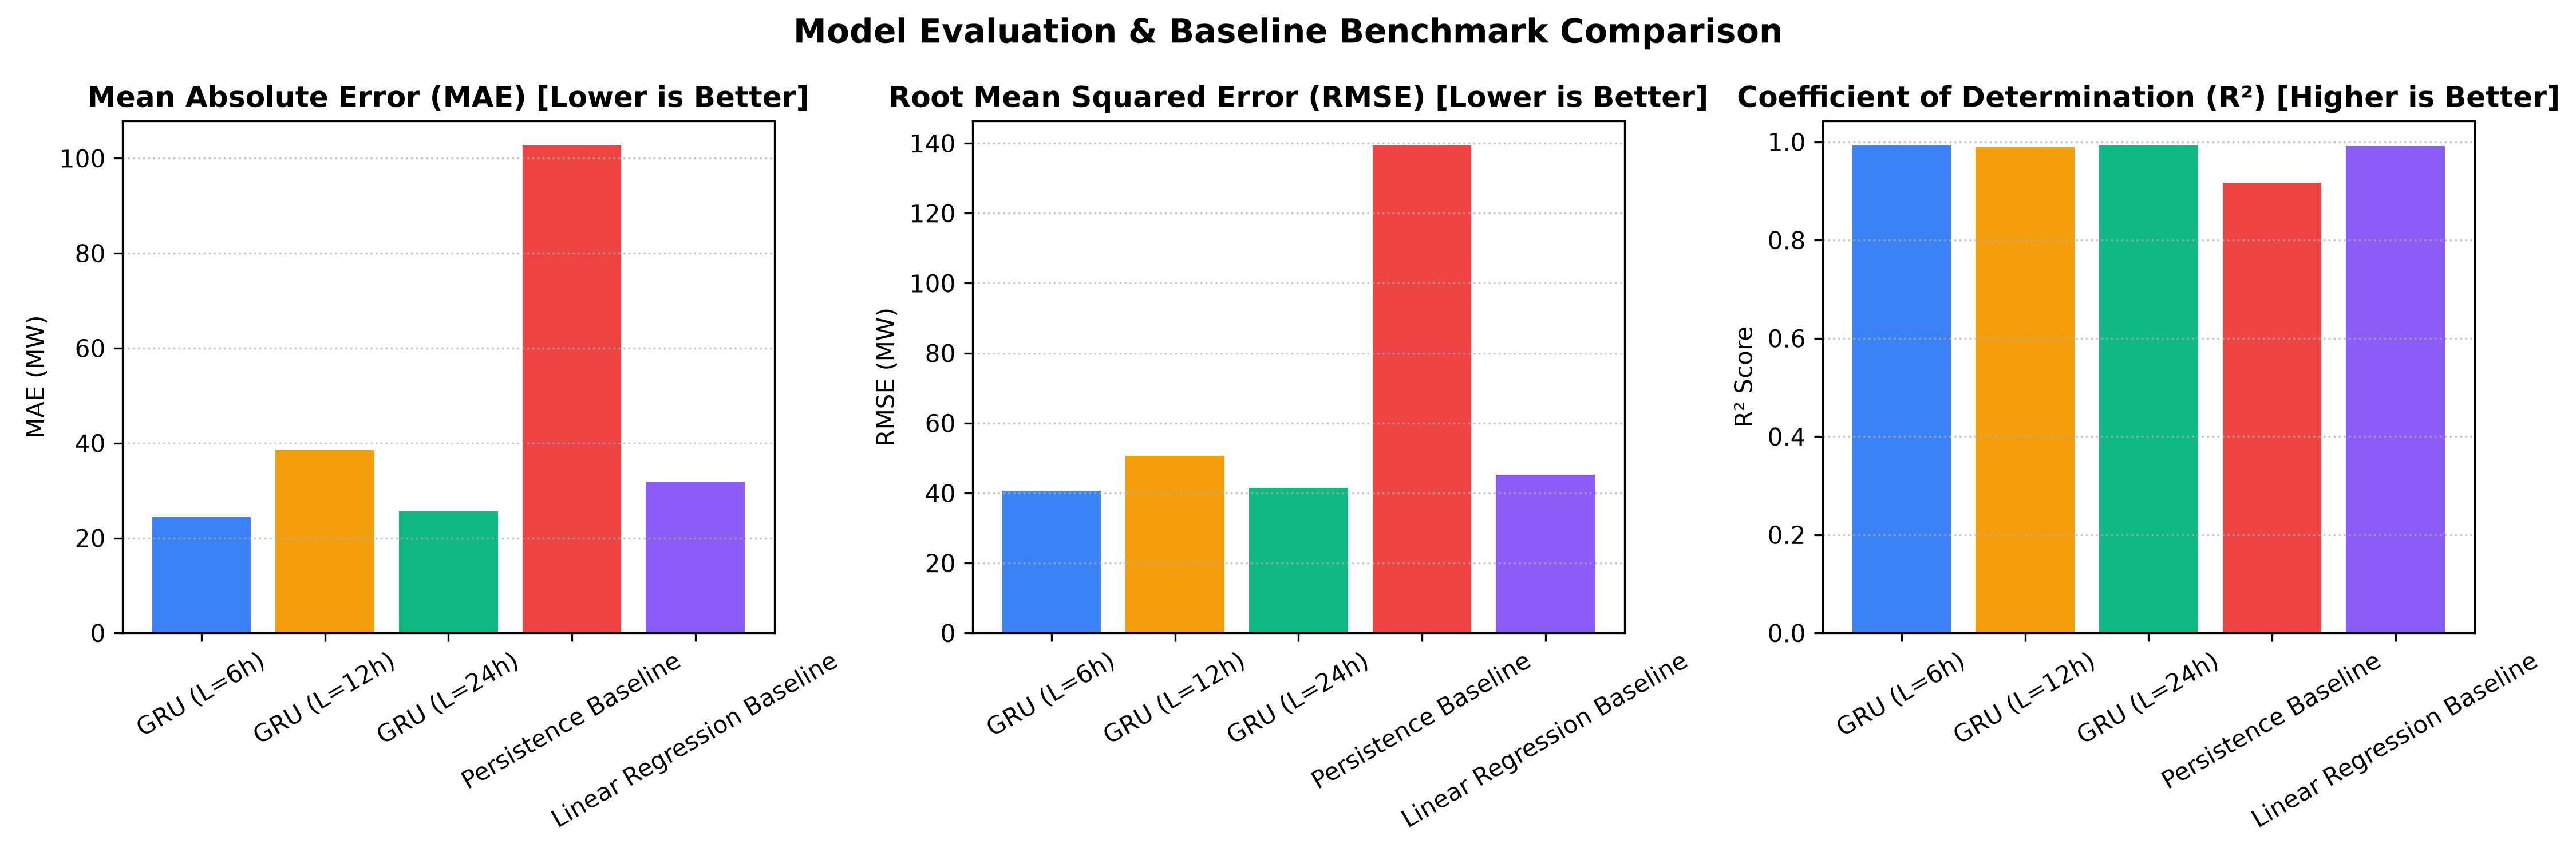
\includegraphics[width=0.88\textwidth]{figures/metrics_comparison_bar.png}
\caption{Comparative performance metrics (MAE, RMSE, and $R^2$) across models.}
\label{fig:metrics}
\end{figure}

\begin{figure}[H]
\centering
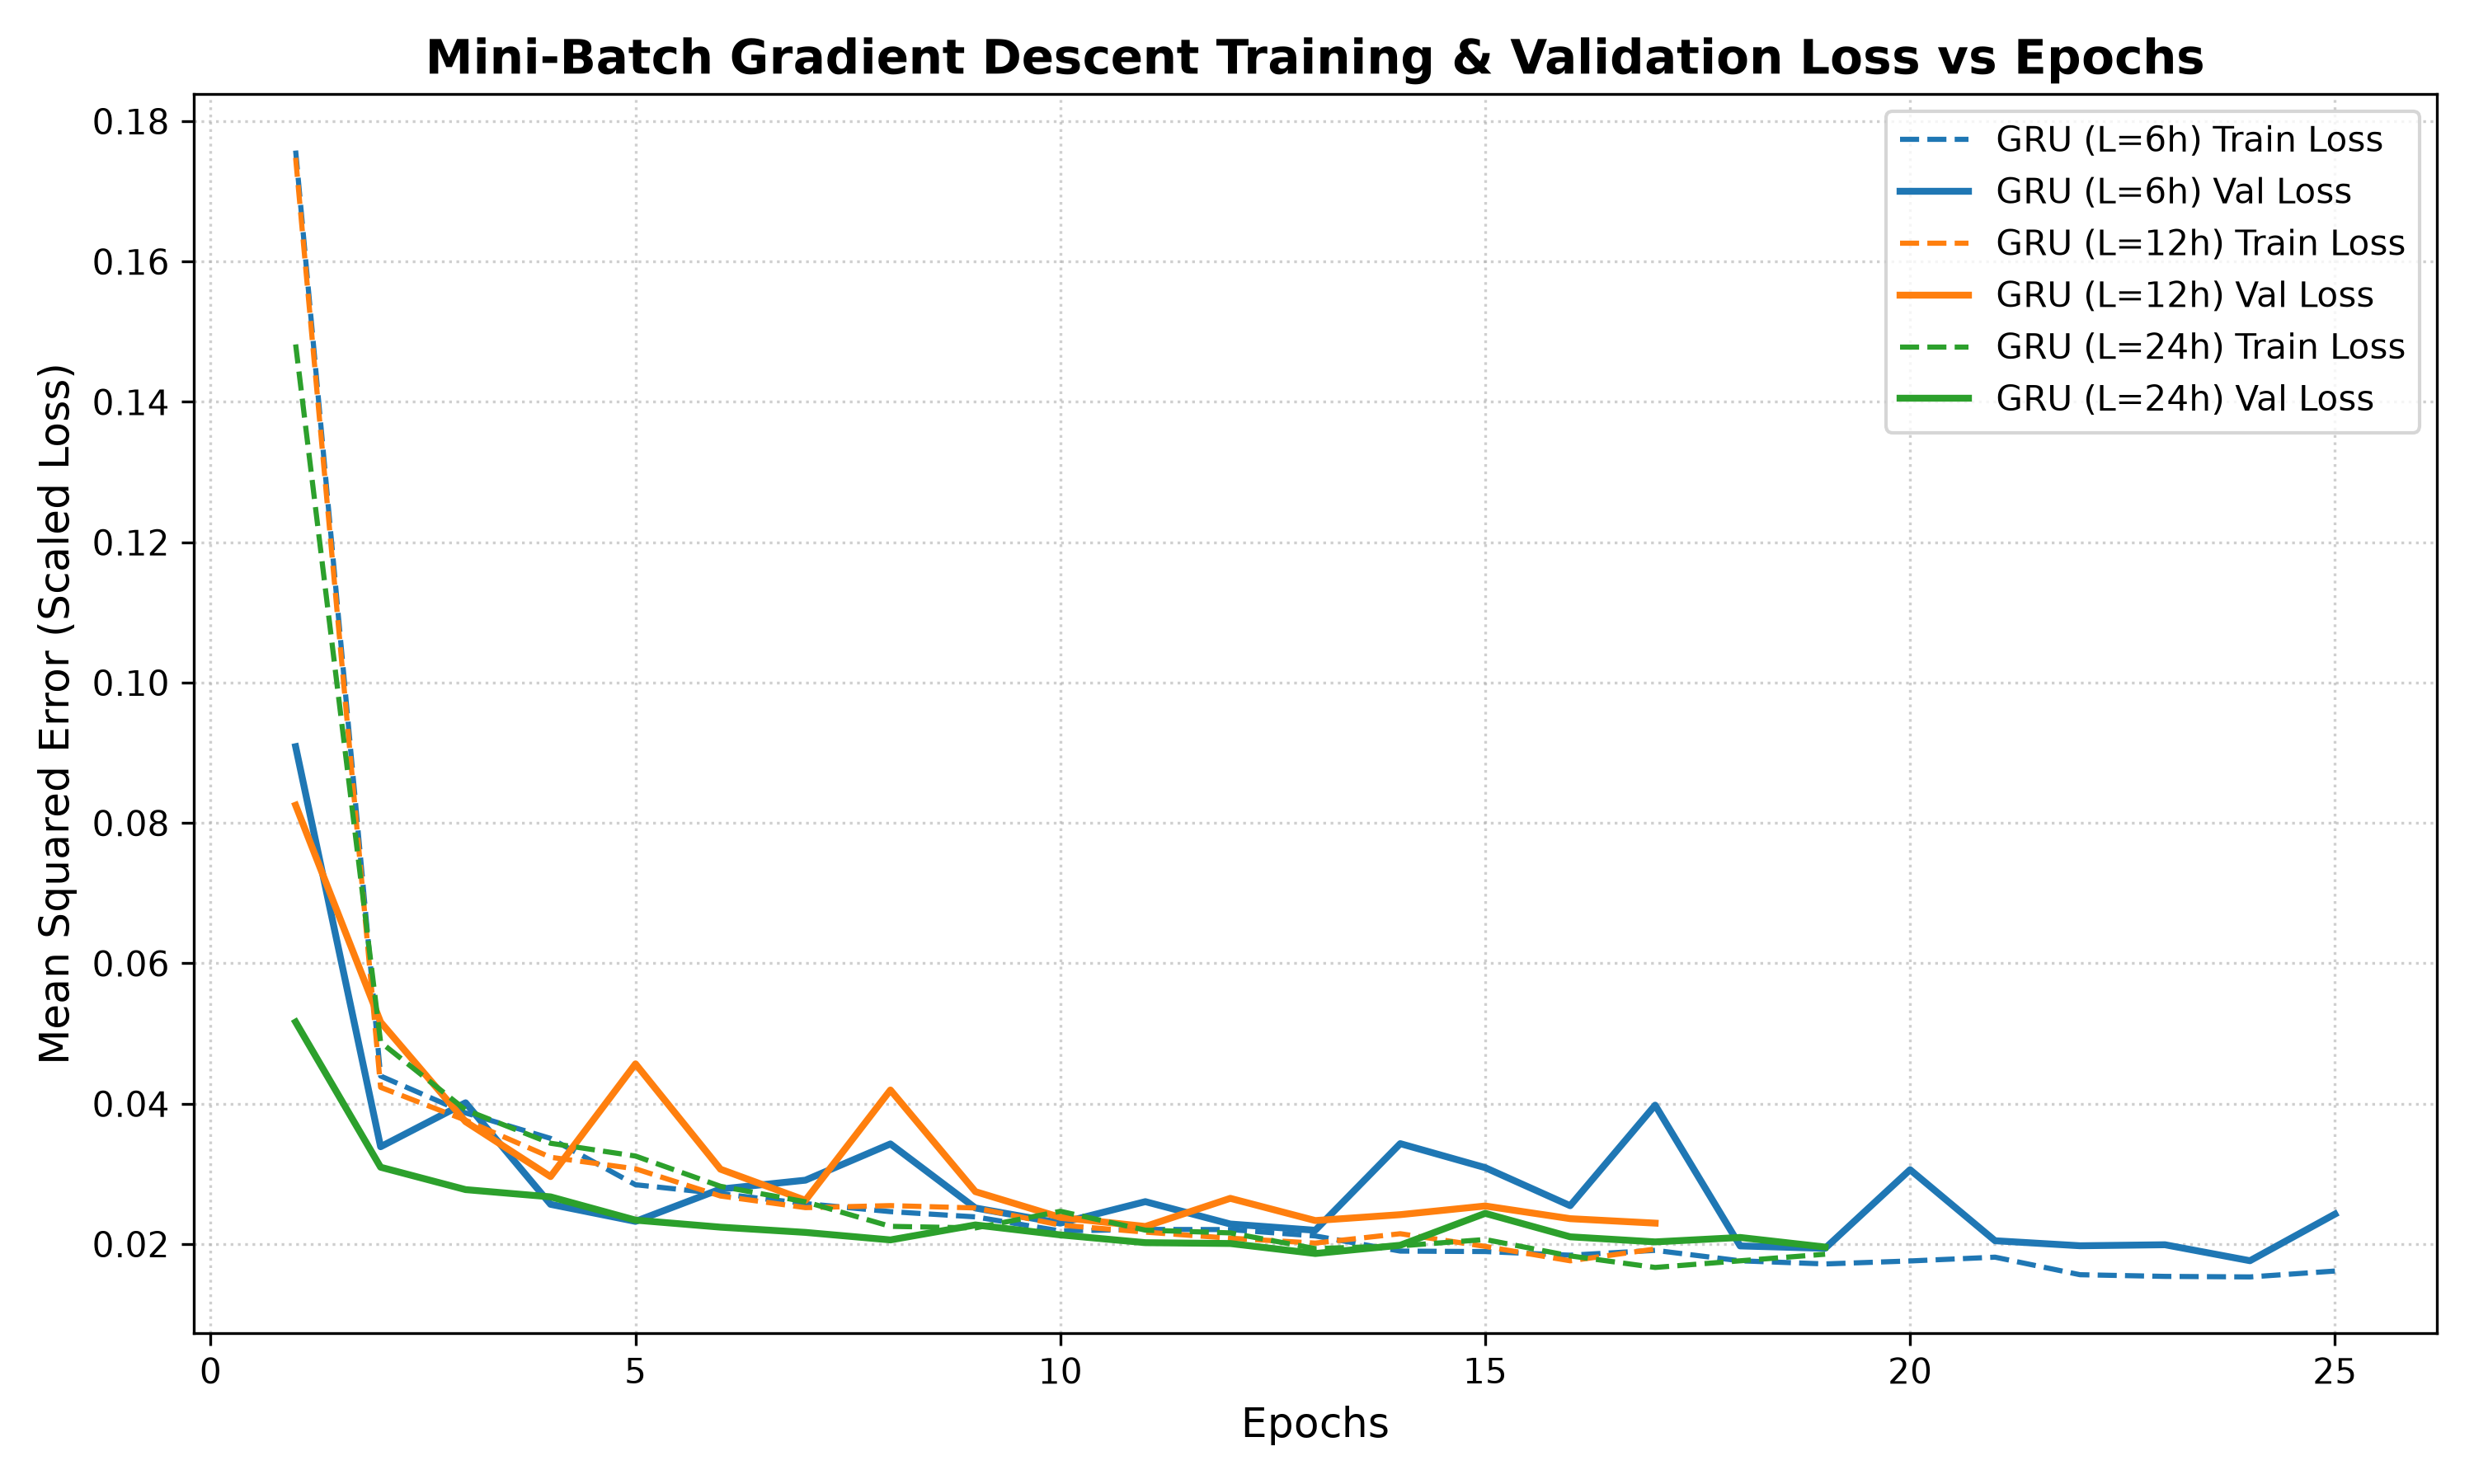
\includegraphics[width=0.85\textwidth]{figures/training_loss_curves.png}
\caption{Mini-Batch Gradient Descent Training and Validation Loss curves across epochs.}
\label{fig:loss}
\end{figure}

\section*{Key Observations and Technical Inferences}
\begin{enumerate}
    \item \textbf{Superiority over Persistence Baseline:} The Persistence baseline demonstrates substantial error ($\text{MAE} = 102.712\text{ MW}$, $\text{RMSE} = 139.378\text{ MW}$) because solar irradiance changes rapidly due to earth rotation and atmospheric shading. GRU models reduced the MAE by over \textbf{76\%}.
    \item \textbf{Sequence Length Comparison ($L=6$ vs $L=12$ vs $L=24$):}
    \begin{itemize}
        \item \textbf{$L=6$ hours:} Achieved the lowest instantaneous MAE (24.469 MW) and RMSE (40.616 MW). Short lookback windows allow the GRU gates to rapidly react to immediate weather fluctuations, sudden cloud cover transients, and recent irradiance dips without carrying unnecessary historical memory from past night hours.
        \item \textbf{$L=24$ hours:} Achieved nearly identical top-tier performance ($\text{MAE} = 25.570\text{ MW}$, $R^2 = 0.9926$), successfully capturing the complete 24-hour diurnal solar cycle.
        \item \textbf{$L=12$ hours:} Produced slightly higher error ($\text{MAE} = 38.491\text{ MW}$) because a 12-hour window splits the day-night boundary inconsistently depending on the starting hour, creating partial diurnal information.
    \end{itemize}
    \item \textbf{Mini-Batch Gradient Descent Stability:} Training with mini-batch updates ($|\mathcal{B}|=32$) and Adam optimizer converged rapidly within 13 to 19 epochs, with validation loss tracking training loss closely, confirming that the 20\% dropout regularization prevented overfitting.
    \item \textbf{Physical Plausibility:} Enforcing zero power output during nighttime hours where solar zenith angle $\theta_z > 90^\circ$ eliminated nocturnal floating errors and matched real grid operations.
\end{enumerate}

\section*{Conclusion}
A Recurrent Neural Network based on Gated Recurrent Units (GRU) was successfully designed, trained with Mini-Batch Gradient Descent, and evaluated for solar power forecasting using Numerical Weather Prediction variables. The GRU network dramatically outperforms simple persistence and linear baselines, achieving an $R^2$ score exceeding 0.99. Comparative sequence length analysis demonstrated that short-term transient windows ($L=6$h) and full diurnal windows ($L=24$h) offer superior feature representations for renewable energy sequence forecasting.

\end{document}
